\documentclass[11pt]{article}

\usepackage[margin=1in]{geometry}
\usepackage[utf8]{inputenc}
\usepackage[T1]{fontenc}
\usepackage[ngerman]{babel}
\usepackage[autostyle=true]{csquotes}
\usepackage{cancel}
\usepackage{enumerate}
\usepackage{textcomp}
\usepackage{calc}
\usepackage{listings}
\usepackage{color}
\usepackage{hyperref}
\usepackage{mdframed}
\usepackage{graphicx}
\usepackage{multirow, tabularx}
\usepackage{tikz}
\usepackage{float}
\usepackage{upquote}
\usepackage{listings}
\usepackage{color}

\usetikzlibrary{calc, arrows, decorations.markings, shapes.symbols, positioning}

\definecolor{editorGray}{rgb}{0.95, 0.95, 0.95}
\definecolor{editorOcher}{rgb}{1, 0.5, 0} % #FF7F00 -> rgb(239, 169, 0)
\definecolor{editorGreen}{rgb}{0, 0.5, 0} % #007C00 -> rgb(0, 124, 0)
\lstdefinelanguage{JavaScript}{
	morekeywords={typeof, new, true, false, catch, function, return, null, catch, switch, var, if, in, while, do, else, case, break},
	morecomment=[s]{/*}{*/},
	morecomment=[l]//,
	morestring=[b]",
	morestring=[b]'
}

\lstdefinelanguage{HTML5}{
	language=html,
	sensitive=true, 
	alsoletter={<>=-},
	otherkeywords={
		% HTML tags
		<html>, <head>, <title>, </title>, <meta, />, </head>, <body>,
		<canvas, \/canvas>, <script>, </script>, </body>, </html>, <!, html>, <style>, </style>, ><
	},  
	ndkeywords={
		% General
		=,
		% HTML attributes
		charset=, id=, width=, height=,
		% CSS properties
		border:, transform:, -moz-transform:, transition-duration:, transition-property:, transition-timing-function:
	},  
	morecomment=[s]{<!--}{-->},
	tag=[s]
}

\lstset{%
	% Basic design
	backgroundcolor=\color{editorGray},
	basicstyle={\small\ttfamily},   
	frame=l,
	% Line numbers
	xleftmargin={0.75cm},
	numbers=left,
	stepnumber=1,
	firstnumber=1,
	numberfirstline=true,
	% Code design   
	keywordstyle=\color{blue}\bfseries,
	commentstyle=\color{darkgray}\ttfamily,
	ndkeywordstyle=\color{editorGreen}\bfseries,
	stringstyle=\color{editorOcher},
	% Code
	language=HTML5,
	alsolanguage=JavaScript,
	alsodigit={.:;},
	tabsize=2,
	showtabs=false,
	showspaces=false,
	showstringspaces=false,
	extendedchars=true,
	breaklines=true,        
	% Support for German umlauts
	literate=%
	{Ö}{{\"O}}1
	{Ä}{{\"A}}1
	{Ü}{{\"U}}1
	{ß}{{\ss}}1
	{ü}{{\"u}}1
	{ä}{{\"a}}1
	{ö}{{\"o}}1
}


\begin{document}
	
	\title{Klausurzusammenfassung Webengineering}
	\author{Florian Kling}
	
	\maketitle
	
	\newpage
	
	
	\section{HTML}
	
		\subsection{Standard HTML Aufbau}
		
		\begin{lstlisting}
			<!DOCTYPE html>
			<html>
				<head>
					<title>Titel der Webseite</title>
				</head>
				<body>
					Hello World!
				</body>
			</html>
		\end{lstlisting}
		
		
		\subsection{Tabellen}
	

			\begin{tabular}{p {0.4 \textwidth}  p {0.6 \textwidth} }
				\begin{center}
					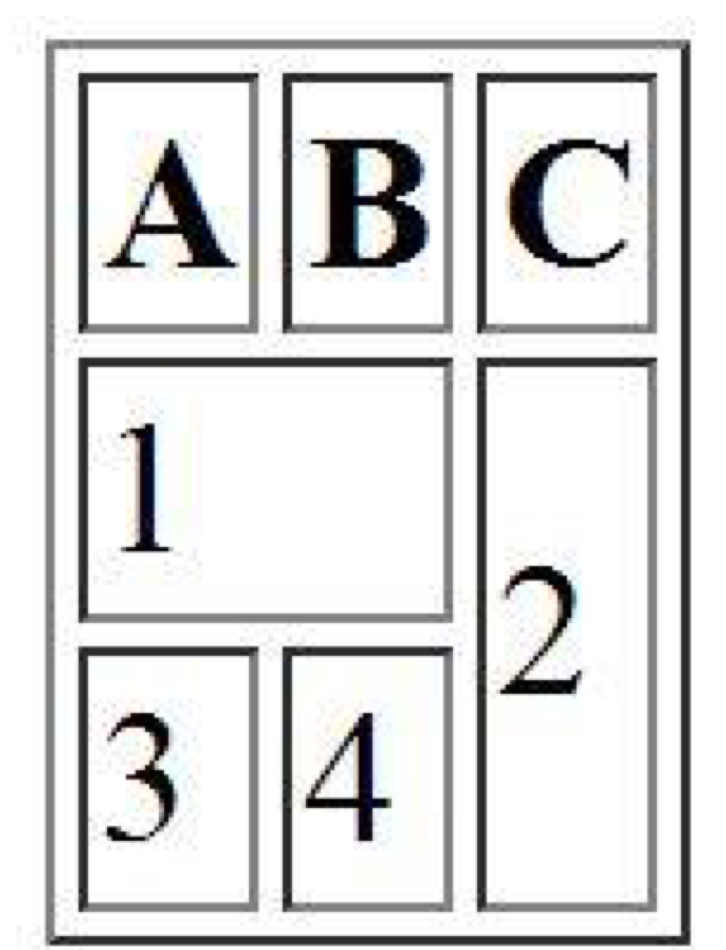
\includegraphics[width=0.7\linewidth]{tabelle}
				\end{center}
			
			& 	
				\begin{lstlisting}
<table border="1">
	<tr>
		<th>A</th>
		<th>B</th>
		<th>C</th>
	</tr>
	<tr>
		<td colspan="2">1</td>
		<td rowspan="2">2</td>
	</tr>
	<tr>
		<td>3</td>
		<td>4</td>
	</tr>
</table>
				\end{lstlisting}
			\end{tabular}
	
		\subsection{Listings}
		
			Es gibt folgende Listen-Style:
			
			\begin{itemize}
				\item <ol type=''1''> $\rightarrow$ numerische Aufzählung
				\item <ol type=''A''> $\rightarrow$ Alphabetische Aufzählung, große Buchstaben
				\item <ol type=''a''> $\rightarrow$ Alphabetische Aufzählung, kleine Buchstaben
				\item <ol type=''I''> $\rightarrow$ große Romanische Ziffern
				\item <ol type=''i''> $\rightarrow$ kleine Romanische Ziffern
			\end{itemize}
			
			Mit der start-Property kann festgelegt werden, mit welchem Zeichen begonnen wird. \newline
			Mit der reverse-Property kann die Aufzählung rückwärts gestaltet werden.
			
	\section{JSP}
	
		\subsection{Java-Bean}
			Eine Bean ist eine Java-Klasse die nur Variablen, getter und setter sowie einen leeren Konstruktor besitzt.
			
		\subsection{Variablen im JSP-Umfeld}
			\begin{itemize}
				\item request $\rightarrow$ Gültigkeitsbereich
				\item response
				\item session $\rightarrow$ Gültigkeitsbereich
				\item pageContext $\rightarrow$ Gültigkeitsbereich
				\item application $\rightarrow$ Gültigkeitsbereich
				\item config
				\item out
			\end{itemize}
		
		\subsection{Gültigkeitsbereiche}
		
		\begin{tabular}{|p {0.2 \textwidth} | p {0.8 \textwidth} |}
			\hline
			\textbf{Name} & \textbf{Bedeutung} \\ \hline
			application & Mit dem Starten der Applikation (bspw. durch Hochfahren des Tomcat) steht dieser Gültigkeitsbereich bis zum Beenden der Applikation zur Verfügung. Dieser ist der umfassendste Gültigkeitsbereich und sollte nur für Attribute genutzt werden, die wirklich für die gesamte Applikation von Bedeutung sind. \\ \hline
			session & Eine Session umfasst eine Nutzersitzung und umfasst mehrere Anfragen. So kann der Status einer Benutzers während der Nutzung gespeichert werden (bspw. ein Warenkorb). Ein ausführliches Kapitel zum Umgang mit Session und dabei zu Beachtendes folgt im weiteren Verlauf des Tutorials. \\ \hline
			request & Dieser Gültigkeitsbereich umfasst genau eine Anfrage eines Nutzers. Aufgrund eines möglichen Forwardings der Anfrage an weitere Servlets bzw. JSPs kann ein Request sich über mehrere JSPs oder Servlets erstrecken. \\ \hline
			page & Dieser Gültigkeitsbereich existiert nur in JSPs und ist nur innerhalb genau einer JSP gültig. Bei einem Forwarding gehen Attribute dieses Gültigkeitsbereichs verloren. \\ \hline
		\end{tabular}
		
						
		\subsection{JSP-Snippets}
		
		
			Oberste Zeile einer JSP-Seite:
			
			\begin{lstlisting}
<%@ page language="java" contentType="text/html; charset=UTF-8" pageEncoding="UTF-8"%> 
			\end{lstlisting}
			
			Einfache Ausgaben
						
			\begin{lstlisting}
<%= 4+5 %>
<%= request.getHeader("User-Agent") %>
			\end{lstlisting}
			
			Java-Umfeld erschaffen	
			
			\begin{lstlisting}
<% JAVA-CODE, bsp. for, if, usw. %>
			\end{lstlisting}
			
			Instanz-Variablen, Methoden deklarieren
			
			\begin{lstlisting}
<%! 
	private int counter = 0;
	public synchronized int next () {			
		counter++;
		return counter; 
	}
%>
			\end{lstlisting}
			
			Kommentare
			
			\begin{lstlisting}
<%-- Kommentar --%>
			\end{lstlisting}
			
			Bean laden
			
			\begin{lstlisting}
<jsp:useBean id="Objektvariable" class="Klassenname"/>
			\end{lstlisting}			
			
			Setter einer Bean aufrufen
			
			\begin{lstlisting}
<jsp:setParameter name="Objektvariable" property="Variable" param="Wert"/>			
			\end{lstlisting}
			
			Getter einer Bean aufrufen
			
			\begin{lstlisting}
<jsp:getParameter name="Objektvariable" property="Variable"/>
			\end{lstlisting}
			
			
		\subsection{JSTL}	
			
			Import-Tag
			
			\begin{lstlisting}
<%@ taglib prefix = "c" uri = "http://java.sun.com/jsp/jstl/core" %>
			\end{lstlisting}
\begin{center}
	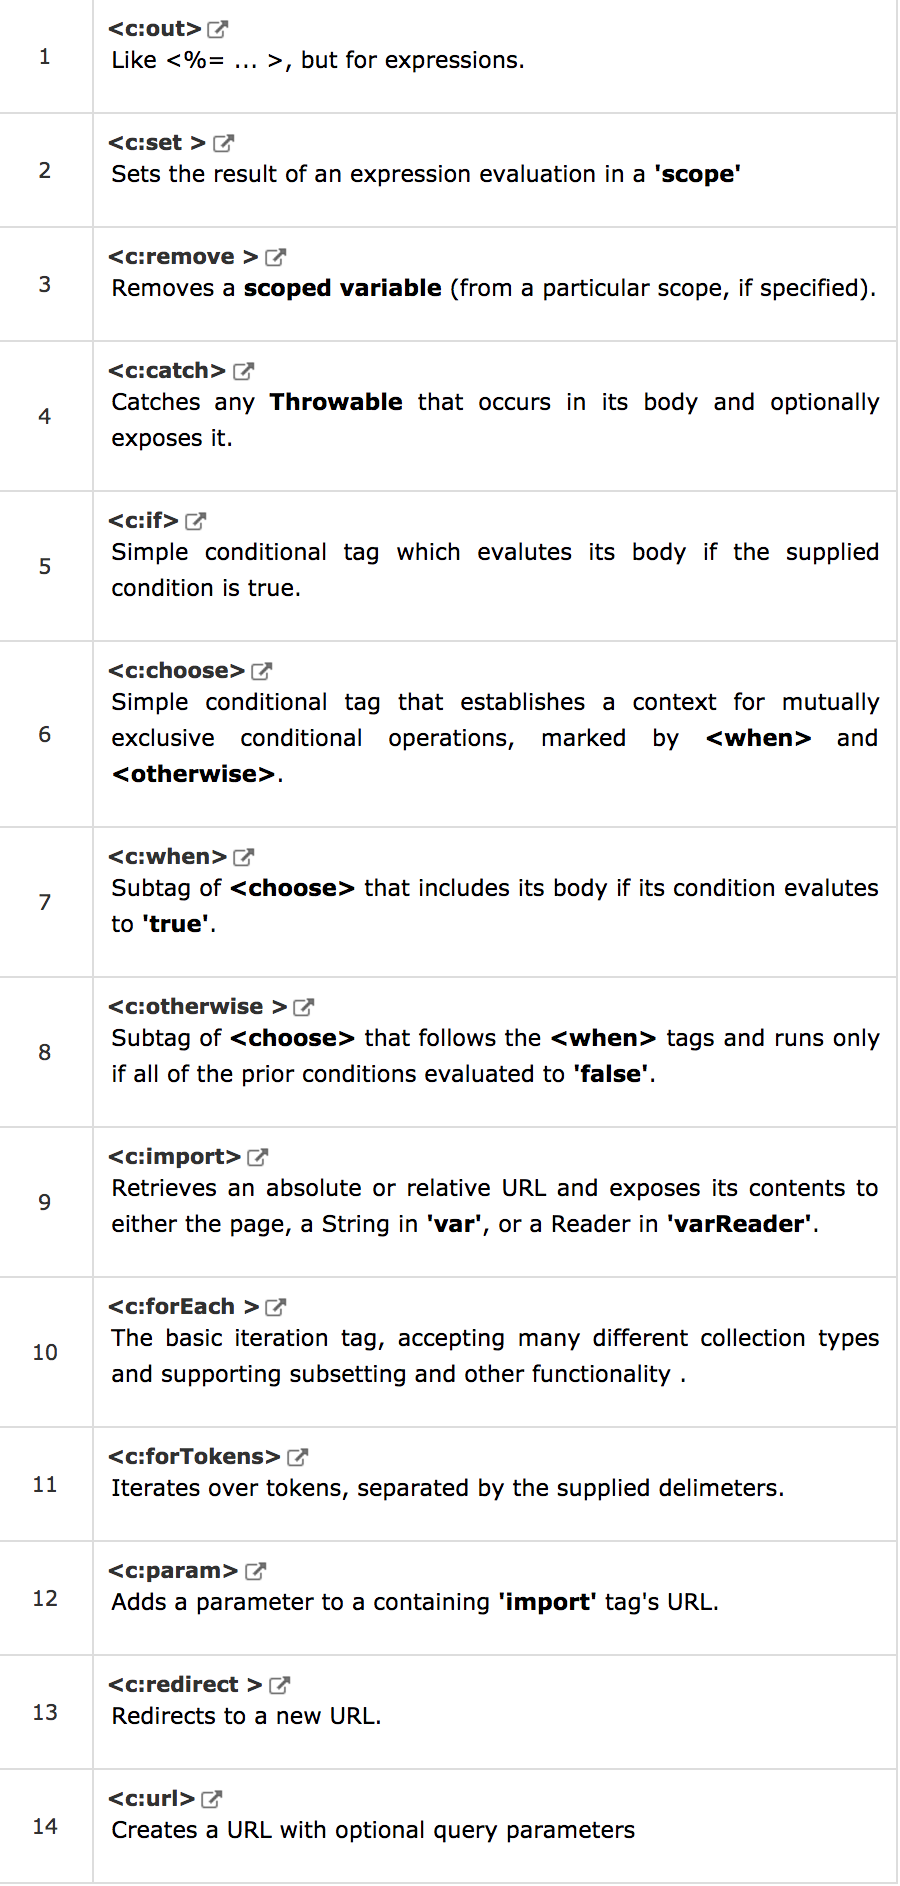
\includegraphics[width=0.7\linewidth]{JSTL_Core}
\end{center}
\begin{center}
	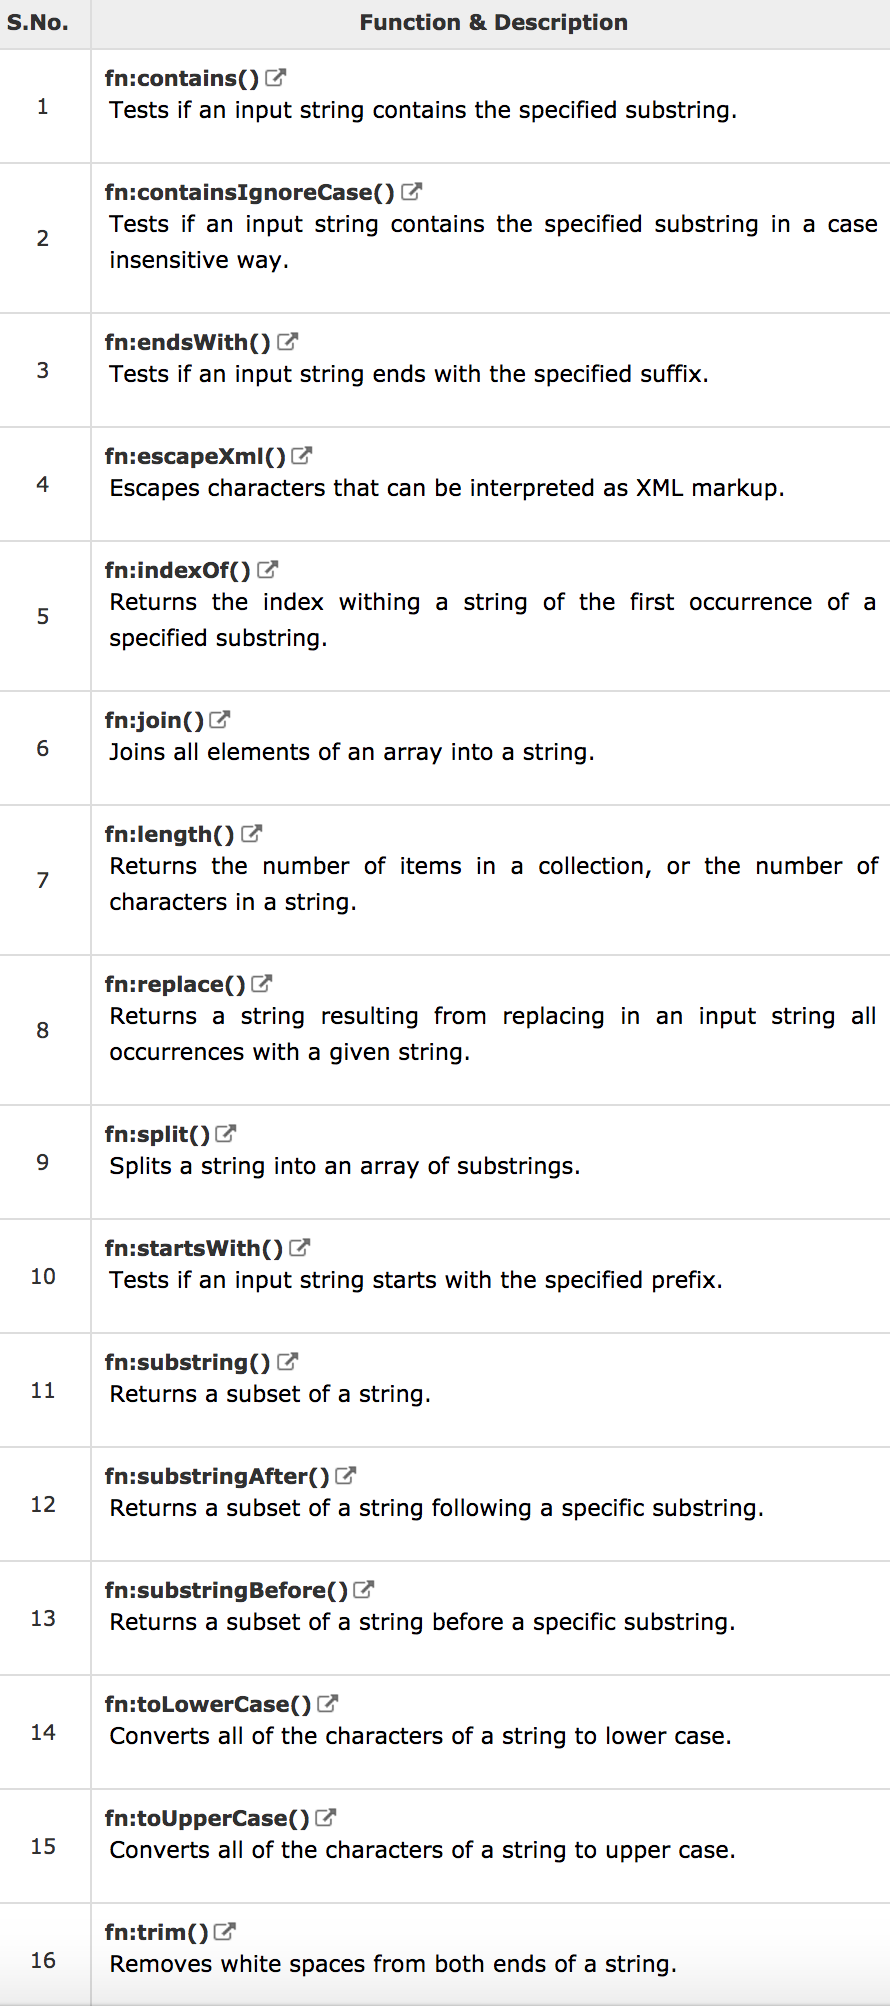
\includegraphics[width=0.7\linewidth]{JSTL_Functions}
\end{center}

	\section{CSS}
		\subsection{CSS Selectors}
			\begin{tabularx}{\textwidth}{|p{0.25\textwidth} | p{0.25\textwidth} | X|}
				\hline
				\textbf{Selector} & \textbf{Example} & \textbf{Example description} \\
				\hline
				\hline
				.class 	& .intro 			& Selects all elements with class="intro" \\
				\hline
				\#id 	& \#firstname 		& Selects the element with id="firstname" \\
				\hline
				\* 		& * 				& Selects all elements \\
				\hline
				element & p 				& Selects all <p> elements \\
				\hline
				element,element & div, p 	& Selects all <div> elements and all <p> elements \\
				\hline
				element element & div p 	& Selects all <p> elements inside <div> elements \\
				\hline
				element>element & div > p 	& Selects all <p> elements where the parent is a <div> element \\
				\hline
				element+element & div + p 	& Selects all <p> elements that are placed immediately after <div> elements \\
				\hline
				element$\sim$element & p $\sim$ ul 	& Selects every <ul> element that are preceded by a <p> element \\
				\hline
				{[attribute]} & [target] 		& Selects all elements with a target attribute \\
				\hline
				{[attribute=value]} & [target=\_blank] 		& Selects all elements with a target="\_blank" \\
				\hline
				{[attribute$\sim$=value]} & [title$\sim$=flower] & Selects all elements with a title attribute containing the word "flower" \\
				\hline
				{[attribute|=value]} & [lang|=en] & Selects all elements with a lang attribute value starting with "en" \\
				\hline
				{[attribute\^=value]} & a[href\^="https"] & Selects every <a> element whose href attribute value begins with "https" \\
				\hline
				{[attribute\$=value]} & a[href\$=".pdf"] & Selects every <a> element whose href attribute value ends with ".pdf" \\
				\hline
				{[attribute*=value]} & a[href*="w3schools"] & Selects every <a> element whose href attribute value contains the substring "schools" \\
				\hline
				:active & a:active & Selects the active link \\
				\hline
				::after & p::after & Insert something after the content of each <p> element \\
				\hline
				::before & p::before & Insert something before the content of each <p> element \\
				\hline
				:checked & input:checked & Selects every checked <input> element \\
				\hline
				:disabled & input:disabled & Selects every disabled <input> element \\
				
				\hline
				:empty & p:empty & Selects every <p> element that has no children (including text nodes) \\
				\hline
				:enabled & input:enabled & Selects every enabled <input> element \\
				\hline
				:first-child & p:first-child & Selects every <p> element that is the first child of its parent \\
				\hline
			\end{tabularx}
			\begin{tabularx}{\textwidth}{|p{0.25\textwidth} | p{0.25\textwidth} | X|}
				
				\hline
				::first-letter & p::first-letter & Selects the first letter of every <p> element \\
				\hline
				::first-line & p::first-line & Selects the first line of every <p> element \\
				\hline
				:first-of-type & p:first-of-type & Selects every <p> element that is the first <p> element of its parent \\
				\hline
				:focus & input:focus & Selects the input element which has focus \\
				\hline
				:hover & a:hover & Selects links on mouse over \\
				\hline
				:in-range & input:in-range & Selects input elements with a value within a specified range \\
				\hline
				:invalid & input:invalid & Selects all input elements with an invalid value \\
				\hline
				:lang(language) & p:lang(it) & Selects every <p> element with a lang attribute equal to "it" (Italian) \\
				\hline
				:last-child & p:last-child & Selects every <p> element that is the last child of its parent \\
				\hline
				:last-of-type & p:last-of-type & Selects every <p> element that is the last <p> element of its parent \\
				\hline
				:link & a:link & Selects all unvisited links \\
				\hline
				:not(selector) & :not(p) & Selects every element that is not a <p> element \\
				\hline
				:nth-child(n) & p:nth-child() & Selects every <p> element that is the second child of its parent \\
				\hline
				:nth-last-child(n) & p:nth-last-child() & Selects every <p> element that is the second child of its parent, counting from the last child \\
				\hline
				:nth-last-of-type(n) & p:nth-last-of-type() & Selects every <p> element that is the second <p> element of its parent, counting from the last child \\
				\hline
				:nth-of-type(n) & p:nth-of-type() & Selects every <p> element that is the second <p> element of its parent \\
				\hline
				:only-of-type & p:only-of-type & Selects every <p> element that is the only <p> element of its parent \\
				\hline
				:only-child & p:only-child & Selects every <p> element that is the only child of its parent \\
				\hline
				:optional & input:optional & Selects input elements with no "required" attribute \\
				\hline
				:out-of-range & input:out-of-range & Selects input elements with a value outside a specified range \\
				\hline
				:read-only & input:read-only & Selects input elements with the "readonly" attribute specified \\
				\hline
				:read-write & input:read-write & Selects input elements with the "readonly" attribute NOT specified \\
				\hline
				:required & input:required & Selects input elements with the "required" attribute specified \\
				\hline
			\end{tabularx}
			\begin{tabularx}{\textwidth}{|p{0.25\textwidth} | p{0.25\textwidth} | X|}
				\hline
				:root & :root & Selects the document's root element \\
				\hline
				::selection & ::selection & Selects the portion of an element that is selected by a user  \\
				\hline
				:target & \#news:target & Selects the current active \#news element (clicked on a URL containing that anchor name) \\
				\hline
				:valid & input:valid & Selects all input elements with a valid value \\
				\hline
				:visited & a:visited & Selects all visited links \\
				\hline
			\end{tabularx}
			
			
\end{document}